\documentclass[12pt]{report}
\usepackage{graphicx}
\usepackage{titling}
\usepackage{amsmath}
\usepackage{amssymb}
\usepackage[latin1]{inputenc}
\usepackage{enumerate}
\usepackage{float}
\usepackage{amsfonts}
\usepackage[usenames,dvipsnames,svgnames,table]{xcolor}
\parindent=0pt
\frenchspacing
\pagestyle{empty}
%\usepackage{}


\newcommand{\HRule}{\rule{\linewidth}{0.5mm}}

\begin{document}

\begin{titlepage}
\begin{center}


\includegraphics[scale=2.0]{../GFX/dtu_logo.pdf}\\[1cm]

\textsc{\LARGE Technical University of Denmark}\\[1.5cm]

\textsc{\Large 02246 Model Checking}\\[0.5cm]


% Title
\HRule \\[0.4cm]
{\huge \bfseries Mandatory Assignment\\Part 1: Discrete Modelling and Verification}\\[0.1cm]
\HRule \\[1.5cm]

% Author and supervisor
\large
\emph{Authors:}
\\[10pt]
Andreas Hallberg \textsc{Kjeldsen}\\
\emph{s092638@student.dtu.dk}
\\[10pt]
Morten Chabert \textsc{Eskesen}\\
\emph{s133304@student.dtu.dk}

\vfill

% Bottom of the page
{\large October 21, 2013}

\end{center}
\end{titlepage}

\chapter*{HJ{\AE}LPE HALL{\O}J}
\begin{tabular}{ | l  c  r | }
	\hline
	CTL	& & Wiki \\ \hline
	$\forall$ & $\equiv$ &  A \\
	$\exists$ & $\equiv$ & E \\
	$\bigcirc$ & $\equiv$ & X \\
	$\Box$ & $\equiv$ & G \\
	$\Diamond$ & $\equiv$ & F \\
	\hline
\end{tabular}
\newpage

\chapter*{Part A: Introductory Problems}
\section*{A1) Practical Problems}

\subsection*{A1.1}
For the FCFS scheduler, we would like to verify that whenever a client has an active job, the scheduler has that job somewhere in its queue. For example, in the case of the first client, we require that whenever $state_1 = 1$, then either $job_1 = 1$ or $job_2 = 1$.

\subsubsection*{A1.1a) Express this as two CTL properties - one for each client}
$client_1$: $AG (state_1 = 1 \Rightarrow \neg(\neg job_1 = 1 \wedge \neg job_2 = 1))$\\
$client_2$: $AG (state_2 = 1 \Rightarrow \neg(\neg job_1 = 2 \wedge \neg job_2 = 2))$

\subsubsection*{A1.1b) Use PRISM to verify whether these properties hold of the FCFS scheduler model}
$P>=1 [G state1=1=>(job1=1)|(job2=1)]$ - Verified.\\
$P>=1 [G state2=1=>(job1=2)|(job2=2)]$ - Verified.

\subsubsection*{A1.1c) Write down two similar properties for the SRT scheduler, explaining your construction}
$client_1$: $AG (state_1 = 1 \Rightarrow job_1 = true)$\\
$client_2$: $AG (state_2 = 1 \Rightarrow job_2 = true)$\\
\\
We require that whenever $state_1 = 1$ then $job_1 = true$ because there should be a job waiting in the queue when the $state_1 = 1$. The same goes for $client_2$.

\subsubsection*{A1.1d) Verify whether they hold of the model}
$P>=1 [G state1=1=>job1=true]$ - Verified.\\
$P>=1 [G state2=1=>job2=true]$ - Verified.


\subsection*{A1.2}
Add another client to the PRISM model of the FCFS scheduler. You will need to modify the $Scheduler$ module to cope with the extra client, but for now do not increase the length of the queue.

\subsubsection*{A1.2a) Explain the changes that you made to the model, and argue why they satisfy the above instructions}
In order for the \emph{Scheduler} to cope with an extra client we first add an extra module called $client_3$ with the same commands as the two other clients with the names of the commands corresponding to $client_3$. We changed the finite range, which $job_1$ and $job_2$ can take their value over to 0\dots3. This does not increase the length of the queue because there is still only two jobs allowed in the queue ($job_1$ and $job_2$). We also added commands create3, serve3 and finish3 and only changed the values according to the number of $client_3$.

\subsubsection*{A1.2b) How many reachable states are in the new model?}
In the new model there are 214 reachable states.

\subsubsection*{A1.2c) What will happen if the queue is full when a client attempts to create a job?}
A client cannot create a job when the queue is full. This is because all the modules synchronize over all action names that appear syntactically in the modules. The commands create1, create2 and create3 are also in scheduler with a guard that specifies that the $job_2 = 0$ for creation of a job to be possible, and $job_2 = 0$ is only true if the queue is empty.

\subsubsection*{A1.2d) Do the properties you have previously verified still hold of the model? If not, why not?}
Yes the properties previously verified still hold in the new model. They do because the clients' states will only be 1 if their job is in the scheduler since the modules are synchronized.

\subsection*{A1.3}
Now modify the $Scheduler$ module so that the queue is of length three.

\subsubsection*{A1.3a) Explain the changes that you made to the model, and argue why they are correct.}
In order to modify the queue to have a length of three we add another job to the queue called $job_3$ which will hold the third job of the queue. We also changed the create commands to have the guard $job_3 = 0$ because now this is the last job in the queue, so when it is 0 there is a place for one more job. Furthermore we added another method for shifting the queue when there is an empty slot. The old command stays in place, but there is now another command with the guard $job_2=0$ \& $job_3>0$ that shifts $job_3$ to $job_2$ so it is moved up in the queue. Since the commands have no action names the commands can always occur \emph{independently} of what any other modules in the systems are doing - just so long as its guard is true.

\subsubsection*{A1.3b) How many reachable states are in the new model?}
In the new model there are 1459 reachable states.

\subsubsection*{A1.3c) Do the properties now hold of the model? If not, why not?}
The properties previously verified do not hold in the new model, because the queue is now of length 3. Which means that a job created by a client could be in scheduled as the last job, i.e. in $job_3$. Example: this would cause (for $client_1$) to have $state_1 = 1$ while $job_3=1$ because the job is at the end of the queue.

\subsubsection*{A1.3d) Can you give an upper bound on the number of reachable states for a model with $n$ clients, and a queue of length $m$?}
????????????????????????????

\subsection*{A1.4}
Consider the CTL properties $\Phi$ and AG $\Phi$, where $\Phi$ is an atomic property.

\subsubsection*{A1.4a) What are their semantics, and how do they differ?}
$AG$ $\Phi$ specifies that from all the paths from this state $\Phi$ should hold. Whereas property $\Phi$ should only hold in that state.

\subsubsection*{A1.4b) Are their semantics different in the version of PRISM that you use?}
The semantics are different in the version of PRISM we use. If the property $\Phi$ should hold in all reachable states it should be written $AG$ $\Phi$. Because if only $\Phi$ has been written as the property - this version of PRISM will only check if the property $\Phi$ holds in the \emph{initial} state.

\subsubsection*{A1.4c) How would you solve the classical model checking problem $M,s \models \Phi$ as a problem of the form $\forall s' : M,s' \models \Phi'$?}
I'll have to think about this.

\subsubsection*{A1.4d) How would you solve the model checking problem $\forall s' : M,s \models \Phi$ as a problem of the form $M,s' \models \Phi'$}
I'll also have to think about this.

\section*{A2) Theoretical Problems}
\subsection*{A2.1}
\begin{figure}[H]
	\centering
	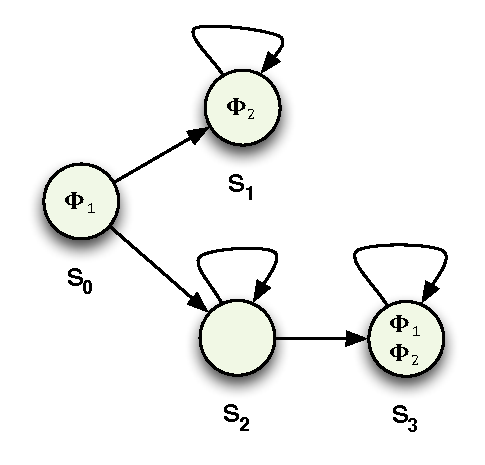
\includegraphics[scale=0.75]{../GFX/ExerciseFigure1.pdf}
	\caption{A transition system}
\end{figure}

Consider the transition system, shown graphically in \textbf{Figure 1}. The states are represented by circles, whose names are shown beneath them, and whose labels are shown inside them. The initial state is $s_0$.

\subsubsection*{A2.1a) Write down this transition system formally, as a tuple $(S,\rightarrow,S_0,AP,L)$}
The transition system will formally be written as:\\
$\langle\{s_0,s_1,s_2,s_3\},\{(s_0 \rightarrow s_1),(s_1 \rightarrow s_1),(s_0 \rightarrow s_2),(s_2 \rightarrow s_2),(s_2 \rightarrow s_3)\},s_0,\{\Phi_1,\Phi_2\},L\rangle$

\subsubsection*{A2.1b) By directly reasoning with the semantics of CTL, determine whether the following properties hold of the state $s_0$}
\begin{enumerate}[i.]
	\item $AF \Phi_2$: Does not hold as $s_2$ can loop indefinitely and therefore $s_3$ is never reached.
	\item $AX \Phi_2$: Does not hold as $s_0 \rightarrow s_2$ isn't allowed.
	\item $EF \Phi_1$: Holds $(s_0 \rightarrow s_2 \rightarrow s_3$).
	\item $A[\Phi_1 U \Phi_2]$: Does not hold as $s_0 \rightarrow s_2$ isn't allowed.
\end{enumerate}

\subsection*{A2.2}
For each of the following pairs of CTL formulae, determine whether (a) they are equivalent, (b) one implies the other, or (c) neither implies the other. Explain your reasoning.
\begin{description}
	\item[A2.2a) $EX$ $EF$ $\Phi$ and $EF$ $EX$ $\Phi$:]
	
	\item[A2.2b) $AX$ $AF$ $\Phi$ and $AF$ $AX$ $\Phi$:]
	
	\item[A2.2c) $AG$ $EF$ $\Phi$ and $EF$ $AG$ $\Phi$:] The first formulae implies the second formulae.\\
	If $AG$ $EF$ $\Phi$ satisfies a transition system then $EF$ $AG$ $\Phi$ will satisfy the same transition system, but not the other way around. Figure A2.2c shows two transition systems, $M1$ and $M2$. $M1$ will satisfy both formulae whereas $M2$ will only satisfy the second formulae.
	\begin{figure}[H]
		\centering
		\begin{tabular}{ l r }
			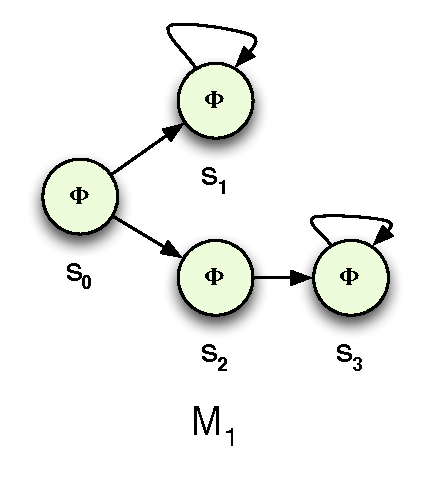
\includegraphics[scale=0.75]{../GFX/Answer-A2-2c-1.pdf}
			& 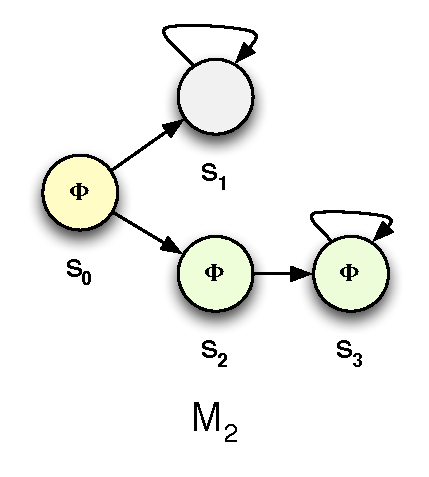
\includegraphics[scale=0.75]{../GFX/Answer-A2-2c-2.pdf}
		\end{tabular}\\
		Figure A2.2c: Two transition systems $M1$ and $M2$.
	\end{figure}
	\textcolor{ForestGreen}{Green} indicates a state that is satisfied both formulae. \textcolor{Goldenrod}{Yellow} indicates a state that is satisfied by just the second formulae. \textcolor{Grey}{Grey} indicates a state that is satisfied by no of the formulae.
	
	\item[A2.2d) $AG$ $(\Phi_1 \wedge \Phi_2)$ and $(AG$ $\Phi_1) \wedge (AG$ $\Phi_2)$:] They're equal.\\
		The first formulae dictates that every state reachable must have $\Phi_1$ and $\Phi_2$. The second formulae firstly dictates that every state reachable must have $\Phi_1$ and secondly dictates that every state reachable must have $\Phi_2$. Thous for both of the formulae to be satisfied every reachable state must have both $\Phi_1$ and $\Phi_2$.\\
		Also it's a distribute law in CTL, see page 330 of the course book.
		
	\item[A2.2e) $EF$ $(\Phi_1 \wedge \Phi_2)$ and $(EF$ $\Phi_1) \wedge (EF$ $\Phi_2)$:]
\end{description}

\subsection*{2A.3}
Write down a CTRL* formula for each of the following properties, which are described in natural language. In each case, argue whether or not the property can also expressed in CTL.

\subsubsection*{2A.3a) There is a path on which $\Phi$ holds infinitely often.}

\subsubsection*{2A.3b) For all paths, $\Phi_1$ holds along the path until $\Phi_2$ holds of a state and $\Phi_3$ holds of the state that immediately follows}

\subsubsection*{2A.3c) There is a path on which either $\Phi_1$ eventually holds or $\Phi_2$ eventually holds}

\subsubsection*{2A.3d) For all paths, either $\Phi_1$ always holds or $\Phi_2$ always holds}

\subsection*{2A.4}
Encode the transition system in \textbf{Figure 1} as a PRISM module, using a variable $s$, such that $0 \leq s \leq 3$, to represent the state. Define $\Phi_1$ and $\Phi_2$ as PRISM labels.

\chapter*{Part B: Intermediate Problems}
\section*{B1) Practical Problems}
\subsection*{B1.1 }
\subsubsection*{(a)}
In order to model a round-robin scheduler from the SRT scheduler we introduce some variables to the \emph{Scheduler} module.
\begin{center}
turn : {[0..2]} init 0; // Who is next?\\
job1time : bool init false; // Has job1 used up its time?\\
job2time : bool init false; // Has job2 used up its time?\\
\end{center}
The turn variable specifies which job is next to be served. When turn=1 the next job to be served is job1.\\
The jobXtime variable specifies if jobX has used up all its serving time in the scheduler. So if jobXtime is true the next job should be served whereas if jobXtime is false this job should be served soon.\\
We also introduce some new commands with no action names in the module. These commands can always occur independently of what any other modules in the system are doing. Its guard just has to be true.
\begin{center}
{[]} job1=true \& job1time=true \& turn=1 $\Rightarrow$ (job1time$'$=false);\\
{[]} job2=true \& job2time=true \& turn=2 $\Rightarrow$ (job2time$'$=false);
\end{center}
These commands are used to switch between the jobs. If job1 has used up all its time in the scheduler but it is now job1s turn in the queue job1time should not be true. It should then be modified to false so it can be served by the scheduler. The same goes for job2.\\
Furthermore we have also modified the serve commands.
\begin{center}
{[serve1]} job1=true \& job2=false $\Rightarrow$ true;\\
{[serve2]} job1=false \& job2=true $\Rightarrow$ true;\\
{[serve1]} job1=true \& job2=true \& turn=1 \& job1time=false $\Rightarrow$ (job1time$'$=true) \& (turn$'$=2);\\
{[serve2]} job1=true \& job2=true \& turn=2 \& job2time=false $\Rightarrow$ (job2time$'$=true) \& (turn$'$=1);
\end{center}
It serves the jobs if there is no other job in the queue. That should not be modified. However it should only serve a job if it is the jobs turn to be served and the job has not used up its time being served. This is in the guard specified as turn has to correspond with the clients number and its jobtime has to be false.
\subsubsection*{(b)}
We have made some additions to the \emph{create} and \emph{finish} commands. The create command now has two different kinds for each client. One is the same as the SRT scheduler. The other command has another guard - turn=0. This command is only used if there has not been any jobs scheduled in the round-robin scheduler before the creation of the new job. When turn=0 there has not been scheduled any jobs yet because turn is initialized as 0 and then turn is only altered between 1 and 2.
\begin{center}
{[create1]} job1=false \& turn>0 $\Rightarrow$ (job$1'$=true);\\
{[create1]} job1=false \& turn=0 $\Rightarrow$ (job$1'$=true) \& (turn$'$=1);\\
{[create2]} job2=false \& turn>0 $\Rightarrow$ (job$2'$=true);\\
{[create2]} job2=false \& turn=0 $\Rightarrow$ (job$2'$=true) \& (turn$'$=2);\\
$\dots$\\
{[finish1]} job1=true $\Rightarrow$ (job$1'$=false) \& (job1time$'$=false);\\
{[finish2]} job2=true $\Rightarrow$ (job$2'$=false) \& (job2time$'$=false);
\end{center}
The finish commands has been altered to also set the variable jobXtime to false. Since the job is now finished its time in the queue should not be specified as used up. It should therefore be sat as false so it does not affect the next job created by the same client.
\subsubsection*{(c)}
In the new model there are 277 reachable states.
\subsubsection*{(d)}
$P>=1 [G state1=1=>job1=true]$ - Verified.\\
$P>=1 [G state2=1=>job2=true]$ - Verified.

\subsection*{2.}
\subsubsection*{(a)}
The \emph{Client} module has been modified with an additional variable called \emph{priority} which can be either 1 or 2. When the priority is 2 the job has a higher priority than a job with priority 1. The create commands have been altered to 10 new ones so the client is able to create jobs with both priority 1 and priority 2.
\begin{center}
priority1 : [1..2] init 1; // Priority of the job\\
{[create1]} state1=0 $\Rightarrow$ (state1$'$=1) \& (task1$'$=1) \& (priority1$'$=1);\\
$\dots$\\
{[create1]} state1=0 $\Rightarrow$ (state1$'$=1) \& (task1$'$=1) \& (priority1$'$=2);\\
$\dots$
\end{center}
\subsubsection*{(b)}
The \emph{Scheduler} module is modified so that when a new job is created and it has a higher priority than a job in the queue it moves ahead of that job. This is done in the module by creating some new create commands in the Scheduler module.
\begin{center}
{[create1]} job2=0 $\Rightarrow$ (job2$'$=1);\\
{[create2]} job2=0 $\Rightarrow$ (job2$'$=2);\\
{[create1]} job2=0 \& priority1=2 \& priority2=1 $\Rightarrow$ (job2$'$=job1) \& (job1$'$=1);\\
{[create2]} job2=0 \& priority2=2 \& priority1=1 $\Rightarrow$ (job2$'$=job1) \& (job1$'$=2);
\end{center}
When a new job is created by any of the clients and it has a priority of 2 and the existing job in the queue has a priority of 1 then the new job moves ahead in the queue and the existing job moves back. If the priorities of the jobs are the same no changes should be made and likewise when the existing job in the queue has a priority of 2 and the newly added job has a priority of 1 then no changes should be made.
\subsubsection*{(c)}
In the new model there 360 reachable states.
\subsubsection*{(d)}
$P>=1 [G state1=1=>(job1=1)|(job2=1)]$ - Verified.\\
$P>=1 [G state2=1=>(job1=2)|(job2=2)]$ - Verified.

\section*{B2) Theoretical Problems}
\subsection*{B2.1}

\begin{figure}[H]
	\centering
	\begin{tabular}{ l r }
		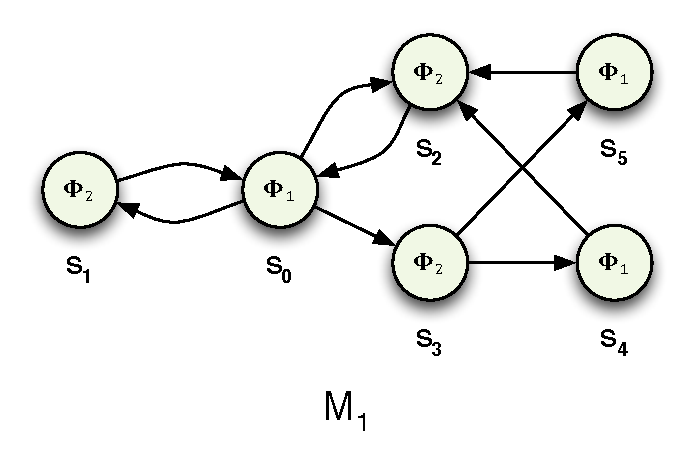
\includegraphics[scale=0.75]{../GFX/ExerciseFigure2-M1.pdf}
		& 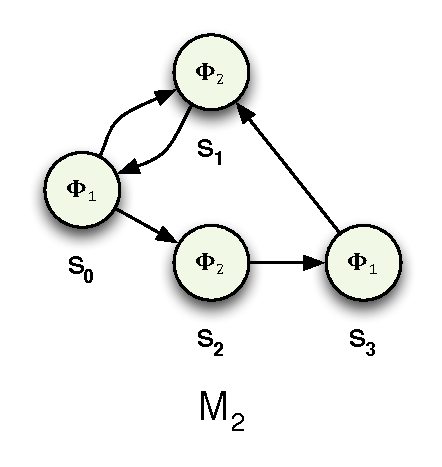
\includegraphics[scale=0.75]{../GFX/ExerciseFigure2-M2.pdf}
	\end{tabular}
	\caption{Two transition systems, $M_1$ and $M_2$}
\end{figure}

\subsubsection*{(a)}

\subsubsection*{(b)}

\subsubsection*{(c)}

\subsubsection*{(d)}

\subsubsection*{(e)}

\subsubsection*{(f)}

\subsection*{2.}
\subsubsection*{(a)}

\subsubsection*{(b)}

\subsubsection*{(c)}

\subsubsection*{(d)}

\chapter*{Part C: Advanced Problems}
\section*{Practical Problems}
We have modified our round-robin scheduler to include priorities. In our specification the scheduler choses the job with the highest priority and it serves it till its finished unless the other job has waited 5 turns. This avoid starvation but it could also keep an important job in the queue while serving a less important job. If the priority is equal the scheduler switches between the jobs in a regular round-robin fashion.\\
\begin{tabular}{ c c c c }
No. & CTL & PRISM notation & Verified \\
1. & $AG (state_1 = 1 \Rightarrow job_1 = true)$ & $P>=1 [G state1=1=>job1=true]$ & $\checkmark$ \\
2. & $AG (state_2 = 1 \Rightarrow job_2 = true)$ & $P>=1 [G state2=1=>job2=true]$ & $\checkmark$ \\
3. & $task_1>0 \Rightarrow AF task_1 = 0$ & $task1>0=>P>=1$ [ F task1=0 ] & $\checkmark$ \\
4. & $task_2>0 \Rightarrow AF task_2 = 0$ & $task2>0=>P>=1$ [ F task2=0 ] & $\checkmark$ \\

\end{tabular}
\end{document}
